\documentclass[11pt,]{article}
\usepackage{lmodern}
\usepackage{amssymb,amsmath}
\usepackage{ifxetex,ifluatex}
\usepackage{fixltx2e} % provides \textsubscript
\ifnum 0\ifxetex 1\fi\ifluatex 1\fi=0 % if pdftex
  \usepackage[T1]{fontenc}
  \usepackage[utf8]{inputenc}
\else % if luatex or xelatex
  \ifxetex
    \usepackage{mathspec}
  \else
    \usepackage{fontspec}
  \fi
  \defaultfontfeatures{Ligatures=TeX,Scale=MatchLowercase}
\fi
% use upquote if available, for straight quotes in verbatim environments
\IfFileExists{upquote.sty}{\usepackage{upquote}}{}
% use microtype if available
\IfFileExists{microtype.sty}{%
\usepackage[]{microtype}
\UseMicrotypeSet[protrusion]{basicmath} % disable protrusion for tt fonts
}{}
\PassOptionsToPackage{hyphens}{url} % url is loaded by hyperref
\usepackage[unicode=true]{hyperref}
\PassOptionsToPackage{usenames,dvipsnames}{color} % color is loaded by hyperref
\hypersetup{
            colorlinks=true,
            linkcolor=Maroon,
            citecolor=Blue,
            urlcolor=Blue,
            breaklinks=true}
\urlstyle{same}  % don't use monospace font for urls
\usepackage[margin=0.75in]{geometry}
\usepackage{longtable,booktabs}
% Fix footnotes in tables (requires footnote package)
\IfFileExists{footnote.sty}{\usepackage{footnote}\makesavenoteenv{long table}}{}
\IfFileExists{parskip.sty}{%
\usepackage{parskip}
}{% else
\setlength{\parindent}{0pt}
\setlength{\parskip}{6pt plus 2pt minus 1pt}
}
\setlength{\emergencystretch}{3em}  % prevent overfull lines
\providecommand{\tightlist}{%
  \setlength{\itemsep}{0pt}\setlength{\parskip}{0pt}}
\setcounter{secnumdepth}{0}
% Redefines (sub)paragraphs to behave more like sections
\ifx\paragraph\undefined\else
\let\oldparagraph\paragraph
\renewcommand{\paragraph}[1]{\oldparagraph{#1}\mbox{}}
\fi
\ifx\subparagraph\undefined\else
\let\oldsubparagraph\subparagraph
\renewcommand{\subparagraph}[1]{\oldsubparagraph{#1}\mbox{}}
\fi

% set default figure placement to htbp
\makeatletter
\def\fps@figure{htbp}
\makeatother

\usepackage[dvipsnames]{xcolor}
\usepackage{pdfpages}
\renewcommand{\arraystretch}{1.08}
\hypersetup{linkcolor=MidnightBlue,urlcolor=MidnightBlue}

\date{}

\begin{document}

\section{Marc meeting: baseline supply
model}\label{marc-meeting-baseline-supply-model}

\textbf{November 10, 2026}

\subsection{1. Overall}\label{overall}

\begin{itemize}
\tightlist
\item
  Selected a provisional national firm-month nested-logit specification
  with negative price slope and fine \(\sigma\)
\item
  Used this specification to implement fixed point Bertrand pricing.
  Audited this
\item
  Built an initial forward-looking entry/exit game with many
  restrictions including exogenous nicotine and demand shocks, five
  fixed brand identities, and private entry/scrap draws.
\item
  Solved the dynamic game and did small calibration exercise (adjust one
  parameter at a time) on FC, sunk entry cost, scrap value standard
  deviation
\end{itemize}

\textbf{Focus: how to ease restrictions in entry/exit game}

\subsubsection{Current baseline at a
glance}\label{current-baseline-at-a-glance}

\begin{longtable}[]{@{}ll@{}}
\toprule
\begin{minipage}[b]{0.32\columnwidth}\raggedright\strut
Component\strut
\end{minipage} & \begin{minipage}[b]{0.62\columnwidth}\raggedright\strut
Implemented version\strut
\end{minipage}\tabularnewline
\midrule
\endhead
\begin{minipage}[t]{0.32\columnwidth}\raggedright\strut
Individually modeled brands\strut
\end{minipage} & \begin{minipage}[t]{0.62\columnwidth}\raggedright\strut
BLU, MISTIC, NJOY, JUUL, VUSE\strut
\end{minipage}\tabularnewline
\begin{minipage}[t]{0.32\columnwidth}\raggedright\strut
Other brands\strut
\end{minipage} & \begin{minipage}[t]{0.62\columnwidth}\raggedright\strut
Passive aggregate fringe, including LOGIC\strut
\end{minipage}\tabularnewline
\begin{minipage}[t]{0.32\columnwidth}\raggedright\strut
Initial date\strut
\end{minipage} & \begin{minipage}[t]{0.62\columnwidth}\raggedright\strut
January 2013; BLU, MISTIC, NJOY active\strut
\end{minipage}\tabularnewline
\begin{minipage}[t]{0.32\columnwidth}\raggedright\strut
Quality\strut
\end{minipage} & \begin{minipage}[t]{0.62\columnwidth}\raggedright\strut
Three nicotine bins × three demand-shock bins\strut
\end{minipage}\tabularnewline
\begin{minipage}[t]{0.32\columnwidth}\raggedright\strut
Industry evolution\strut
\end{minipage} & \begin{minipage}[t]{0.62\columnwidth}\raggedright\strut
JUUL/VUSE entry; absorbing exit; no fringe promotion\strut
\end{minipage}\tabularnewline
\begin{minipage}[t]{0.32\columnwidth}\raggedright\strut
Completed solves\strut
\end{minipage} & \begin{minipage}[t]{0.62\columnwidth}\raggedright\strut
Stationary January 2013 market size and fringe benchmark\strut
\end{minipage}\tabularnewline
\begin{minipage}[t]{0.32\columnwidth}\raggedright\strut
Payoff calibration\strut
\end{minipage} & \begin{minipage}[t]{0.62\columnwidth}\raggedright\strut
Common fixed cost; exponential entry cost; normal net scrap\strut
\end{minipage}\tabularnewline
\bottomrule
\end{longtable}

\subsubsection{Reading guide}\label{reading-guide}

Pages 2--3: demand and pricing. Pages 4--6: roster, state, cost, and
fringe restrictions. Pages 7--8: timing, private payoffs, and event
definitions. Page 9: calibration and fit. Page 10: discussion priorities
and brief audit summary.

Detailed checks and figures follow in the appendix. The
\href{marc_mtg_2026-11-10.pdf}{full working notes} retain the
specification tables and decision history. This document describes the
implemented baseline rather than superseded anonymous-slot proposals,
and adds the subsequent coordinate-calibration results.

\clearpage

\subsection{2. Demand carried into the supply
model}\label{demand-carried-into-the-supply-model}

\[
\log(s_{it}/s_{0t})=c+\alpha p_{it}+\beta_a a_{it}
+\sigma\log(s_{it}/s_{gt})+\xi_{it}.
\]

\begin{longtable}[]{@{}ll@{}}
\toprule
Element & Selected specification\tabularnewline
\midrule
\endhead
Price & Liquid-volume-weighted real dollars per mL\tabularnewline
Control & Delivered nicotine concentration \(a_{it}\)\tabularnewline
Excluded instruments & Sales-weighted state tax + annual incumbent
count\tabularnewline
Endogenous variables & Price and within-nest log share\tabularnewline
Market-size definition & Constant consumption intensity × adult
population\tabularnewline
Sample / uncertainty & 528 observations, 132 months; month-clustered
SE\tabularnewline
\bottomrule
\end{longtable}

\[
\widehat\alpha=-0.334\;(0.039),\quad
\widehat\beta_a=0.110\;(0.009),\quad
\widehat\sigma=0.869\;(0.237).
\]

Demand estimation retains the annual greater-than-7\% incumbent
classification.

\subsubsection{Why this provisional
specification?}\label{why-this-provisional-specification}

\begin{itemize}
\tightlist
\item
  Its instrument family has admissible \(\sigma\) in \textbf{24/24}
  runs; \textbf{20/24} also have negative \(\alpha\).
\item
  Expanded Gandhi--Houde constructions give some admissible alternatives
  and smaller SEs, but was not smoking gun.
\end{itemize}

\subsubsection{Unresolved restrictions}\label{unresolved-restrictions}

Instrument exclusion, the negative conditional tax--price relationship,
and market-size validity remain unresolved. Sigma's conventional 95\%
interval extends above one.

\clearpage

\hypertarget{static-bertrand-pricing-and-recovered-profits}{\subsection{3.
Static Bertrand pricing and recovered
profits}\label{static-bertrand-pricing-and-recovered-profits}}

Each active brand chooses its own price holding rivals' prices and
nonprice states fixed:

\[
\pi_i(p,\Omega)=(p_i-mc_i)M s_i(p,\Omega)-FC.
\]

Here \(\Omega\) is the public industry state: which focal brands are
active, each active brand's nicotine and \(\xi\) bins, and whether
JUUL/VUSE have never entered or have permanently exited. Costs, fringe
utility, market size, and demand coefficients are fixed inputs in this
stationary baseline. Private entry-cost and scrap draws are not part of
\(\Omega\).

Define \(A_i(p)=\frac{1-\sigma s_{i\mid g}(p)}{1-\sigma}-s_i(p)\)

The manual markup fixed point and scaled FOC are

\[
p_i=mc_i-\frac{1}{\alpha A_i(p)},\qquad
1+\alpha(p_i-mc_i)A_i(p)=0.
\]

Demand residuals are inverted from observed shares; historical MC is
inverted from observed-price FOCs. At simulated states, static pricing
supplies variable profit \((p_i-mc_i)Ms_i\), before subtracting dynamic
fixed cost.
\protect\hyperlink{appendix-g-from-observed-shares-to-simulated-profits}{Step-by-step
explanation in Appendix G}.

\subsubsection{Assumptions}\label{assumptions}

\begin{itemize}
\tightlist
\item
  Constant mc
\item
  Fringe is a passive competitor - hold their mean utility \(\delta_F\)
  fixed. Do not separately solve for a fringe price or let it respond to
  incumbents.
\end{itemize}

\subsubsection{Audit summary}\label{audit-summary}

Checked different starting prices and damping; observed versus solved
prices; price, MC, and markup graphs; convergence/FOC residuals; profit
curves; simultaneous versus sequential updates. See Appendix A/D.

\clearpage

\textbf{Moving to dynamic supply}

\subsection{4. Key restrictions: predetermined incumbent
roster}\label{key-restrictions-predetermined-incumbent-roster}

\textbf{Track BLU, MISTIC, NJOY, JUUL, and VUSE individually.} This is
the union of the four highest cumulative-volume brands and annual sales
leaders over 2013--2023. LOGIC is placed in the fringe to limit to five.

I did this to bound the state space. It does not allow for industry
turnover. I continue modeling each selected brand individually while it
operates, regardless of market share.

If I continually admit the top-five, this leads to 12-13 brands.

\subsubsection{Question}\label{question}

Unclear how to maintain the five-firm cap while allowing rising fringe
firms to join, whether or not I need to model in an incumbent's value
function that they could be demoted to fringe? Or having promotion in
fringe value function? Scrap value, as of now, is paid on actual shut
down.

\clearpage

\subsection{5. Key restrictions: quality states and
transitions}\label{key-restrictions-quality-states-and-transitions}

Nicotine \(a\) and recovered demand shock \(\xi\) each have three pooled
quantile bins, represented by \textbf{within-bin medians}:

\[
\Pr(a',\xi'\mid a,\xi)=P_a(a'\mid a)P_\xi(\xi'\mid\xi).
\]

\begin{longtable}[]{@{}ll@{}}
\toprule
\begin{minipage}[b]{0.32\columnwidth}\raggedright\strut
Assumptions\strut
\end{minipage} & \begin{minipage}[b]{0.62\columnwidth}\raggedright\strut
Reason / alternative deferred\strut
\end{minipage}\tabularnewline
\midrule
\endhead
\begin{minipage}[t]{0.32\columnwidth}\raggedright\strut
Exogenous nicotine and \(\xi\)\strut
\end{minipage} & \begin{minipage}[t]{0.62\columnwidth}\raggedright\strut
Omits quality investment\strut
\end{minipage}\tabularnewline
\begin{minipage}[t]{0.32\columnwidth}\raggedright\strut
3 × 3 quantile bins\strut
\end{minipage} & \begin{minipage}[t]{0.62\columnwidth}\raggedright\strut
Nine occupied cells, each with at least 27 departures. Finer grids have
thin rows; equally spaced 3×3 leaves two cells empty.\strut
\end{minipage}\tabularnewline
\begin{minipage}[t]{0.32\columnwidth}\raggedright\strut
Within-bin medians for both variables\strut
\end{minipage} & \begin{minipage}[t]{0.62\columnwidth}\raggedright\strut
Consistent representative values; Within-cell means are an
alternative.\strut
\end{minipage}\tabularnewline
\begin{minipage}[t]{0.32\columnwidth}\raggedright\strut
Pooled transition matrices across brands\strut
\end{minipage} & \begin{minipage}[t]{0.62\columnwidth}\raggedright\strut
Short histories and incomplete joint-state support make firm-specific
estimation difficult; MARKTEN has 11 consecutive transitions overall.
Pooling does not prove common behavior.\strut
\end{minipage}\tabularnewline
\begin{minipage}[t]{0.32\columnwidth}\raggedright\strut
Separate independent \(a\) and \(\xi\) processes\strut
\end{minipage} & \begin{minipage}[t]{0.62\columnwidth}\raggedright\strut
Follows initial plan; 12 free probabilities rather than 72 for
unrestricted joint nine-state transitions. Fewer probabilities to
estimate\strut
\end{minipage}\tabularnewline
\bottomrule
\end{longtable}

\subsubsection{Data support and
persistence}\label{data-support-and-persistence}

The exercise uses 540 incumbent-roster observations and 531
adjacent-month pairs. Nicotine monthly stay probabilities are about
\textbf{97\%, 94\%, 98\%}; \(\xi\) persistence is \textbf{85\%, 74\%,
89\%}. Roster selection may affect transition estimates.

Representative nicotine values: 10.396, 15.396, 29.606. Representative
\(\xi\): −0.685, −0.039, 0.743. Full matrices and bin-support
comparisons are in Appendix B.

\clearpage

\hypertarget{key-restrictions-costs-fringe-and-market-size}{\subsection{6.
Key restrictions: costs, fringe, and market
size}\label{key-restrictions-costs-fringe-and-market-size}}

\begin{longtable}[]{@{}ll@{}}
\toprule
\begin{minipage}[b]{0.32\columnwidth}\raggedright\strut
Baseline restriction\strut
\end{minipage} & \begin{minipage}[b]{0.62\columnwidth}\raggedright\strut
Evidence / reason alternatives deferred\strut
\end{minipage}\tabularnewline
\midrule
\endhead
\begin{minipage}[t]{0.32\columnwidth}\raggedright\strut
Constant brand-specific MC\strut
\end{minipage} & \begin{minipage}[t]{0.62\columnwidth}\raggedright\strut
Historical within-brand median avoids an additional cost state/process.
Not empirically supported.\strut
\end{minipage}\tabularnewline
\begin{minipage}[t]{0.32\columnwidth}\raggedright\strut
Brand-specific MC upon entry\strut
\end{minipage} & \begin{minipage}[t]{0.62\columnwidth}\raggedright\strut
JUUL/VUSE use their assigned medians, known before entry and retained
afterward.\strut
\end{minipage}\tabularnewline
\begin{minipage}[t]{0.32\columnwidth}\raggedright\strut
Constant January 2013 fringe total utility\strut
\end{minipage} & \begin{minipage}[t]{0.62\columnwidth}\raggedright\strut
We must tell firms what fringe competition looks like in future. Using
the median fringe utility from full sample made the fringe much more
attractive relative to incumbents (implausible)\strut
\end{minipage}\tabularnewline
\begin{minipage}[t]{0.32\columnwidth}\raggedright\strut
Constant January 2013 market size\strut
\end{minipage} & \begin{minipage}[t]{0.62\columnwidth}\raggedright\strut
Avoids solving changing market sizes for this trial.\strut
\end{minipage}\tabularnewline
\begin{minipage}[t]{0.32\columnwidth}\raggedright\strut
Common constant \(FC\)\strut
\end{minipage} & \begin{minipage}[t]{0.62\columnwidth}\raggedright\strut
Hard to estimate because in this version, we only have two entry events
among the five brands\strut
\end{minipage}\tabularnewline
\bottomrule
\end{longtable}

\subsubsection{Assigned MC: real dollars per
mL}\label{assigned-mc-real-dollars-per-ml}

\begin{longtable}[]{@{}rrrrr@{}}
\toprule
BLU & MISTIC & NJOY & JUUL & VUSE\tabularnewline
\midrule
\endhead
7.653 & 1.017 & 3.320 & 6.887 & 3.293\tabularnewline
\bottomrule
\end{longtable}

IN some months, MISTIC observations imply negative MC. Cost figures are
in Appendix C.

\subsubsection{Fringe constant period choice
matters}\label{fringe-constant-period-choice-matters}

\begin{longtable}[]{@{}lrr@{}}
\toprule
\begin{minipage}[b]{0.38\columnwidth}\raggedright\strut
January monthly variable profit\strut
\end{minipage} & \begin{minipage}[b]{0.27\columnwidth}\raggedleft\strut
Median fringe utility\strut
\end{minipage} & \begin{minipage}[b]{0.27\columnwidth}\raggedleft\strut
January fringe utility\strut
\end{minipage}\tabularnewline
\midrule
\endhead
\begin{minipage}[t]{0.38\columnwidth}\raggedright\strut
BLU\strut
\end{minipage} & \begin{minipage}[t]{0.27\columnwidth}\raggedleft\strut
\$54\strut
\end{minipage} & \begin{minipage}[t]{0.27\columnwidth}\raggedleft\strut
\$142,325\strut
\end{minipage}\tabularnewline
\begin{minipage}[t]{0.38\columnwidth}\raggedright\strut
MISTIC\strut
\end{minipage} & \begin{minipage}[t]{0.27\columnwidth}\raggedleft\strut
\$331\strut
\end{minipage} & \begin{minipage}[t]{0.27\columnwidth}\raggedleft\strut
\$714,728\strut
\end{minipage}\tabularnewline
\begin{minipage}[t]{0.38\columnwidth}\raggedright\strut
NJOY\strut
\end{minipage} & \begin{minipage}[t]{0.27\columnwidth}\raggedleft\strut
\$130\strut
\end{minipage} & \begin{minipage}[t]{0.27\columnwidth}\raggedleft\strut
\$327,198\strut
\end{minipage}\tabularnewline
\bottomrule
\end{longtable}

\clearpage

\subsection{7. Dynamic timing and the option to
wait}\label{dynamic-timing-and-the-option-to-wait}

\subsubsection{Monthly sequence}\label{monthly-sequence}

\begin{enumerate}
\def\labelenumi{\arabic{enumi}.}
\tightlist
\item
  Observe public state: active identities and quality states, plus fixed
  cost/demand primitives.
\item
  Active firms play the static pricing game and earn profit minus
  \(FC\).
\item
  Active firms privately observe scrap draws; never-entered candidates
  privately observe entry costs. Exit/entry decisions are simultaneous.
\item
  Exit pays scrap now and removes the brand next month. Entry cost is
  paid now; initial quality is revealed after commitment, with
  operations next month.
\item
  Continuing qualities transition independently. A new entrant receives
  its initial draw without an extra transition before first operation.
\end{enumerate}

\clearpage

\subsection{8. Key restrictions: private payoffs and observed
events}\label{key-restrictions-private-payoffs-and-observed-events}

\begin{longtable}[]{@{}ll@{}}
\toprule
\begin{minipage}[b]{0.32\columnwidth}\raggedright\strut
Baseline restriction\strut
\end{minipage} & \begin{minipage}[b]{0.62\columnwidth}\raggedright\strut
Reason / qualification\strut
\end{minipage}\tabularnewline
\midrule
\endhead
\begin{minipage}[t]{0.32\columnwidth}\raggedright\strut
Exponential entry cost, common mean \(\mu_E\)\strut
\end{minipage} & \begin{minipage}[t]{0.62\columnwidth}\raggedright\strut
One positive-support parameter; SD equals mean.\strut
\end{minipage}\tabularnewline
\begin{minipage}[t]{0.32\columnwidth}\raggedright\strut
Normal net scrap: mean zero, SD \(\sigma_S\)\strut
\end{minipage} & \begin{minipage}[t]{0.62\columnwidth}\raggedright\strut
Allows liquidation gains or shutdown costs; only dispersion is
free.\strut
\end{minipage}\tabularnewline
\begin{minipage}[t]{0.32\columnwidth}\raggedright\strut
Normalize mean net scrap to zero\strut
\end{minipage} & \begin{minipage}[t]{0.62\columnwidth}\raggedright\strut
Restricts payoff location alongside operating/entry-cost levels. Does
not prove identification or claim observed mean liquidation is
zero.\strut
\end{minipage}\tabularnewline
\begin{minipage}[t]{0.32\columnwidth}\raggedright\strut
Fresh independent private draws across firms/months\strut
\end{minipage} & \begin{minipage}[t]{0.62\columnwidth}\raggedright\strut
No persistent private type or learning state. Draws reveal no future
public shocks.\strut
\end{minipage}\tabularnewline
\begin{minipage}[t]{0.32\columnwidth}\raggedright\strut
Annual discount 0.95\strut
\end{minipage} & \begin{minipage}[t]{0.62\columnwidth}\raggedright\strut
Fixed, not estimated; monthly
\(\beta=0.95^{1/12}\approx0.995735\).\strut
\end{minipage}\tabularnewline
\begin{minipage}[t]{0.32\columnwidth}\raggedright\strut
Common entrant initial-state distribution\strut
\end{minipage} & \begin{minipage}[t]{0.62\columnwidth}\raggedright\strut
Liquid-volume weights from newly qualifying incumbents' first
incumbent-year windows, aligned with the original entrant-MC exercise.
Successful incumbents are imperfect newborn-firm proxies.\strut
\end{minipage}\tabularnewline
\begin{minipage}[t]{0.32\columnwidth}\raggedright\strut
Initial quality revealed after commitment\strut
\end{minipage} & \begin{minipage}[t]{0.62\columnwidth}\raggedright\strut
Integrate over quality before entering; a privately observed poor
initial draw cannot explain delay in this version.\strut
\end{minipage}\tabularnewline
\begin{minipage}[t]{0.32\columnwidth}\raggedright\strut
January 2013 initialization\strut
\end{minipage} & \begin{minipage}[t]{0.62\columnwidth}\raggedright\strut
BLU/MISTIC/NJOY already active; births left-censored. JUUL/VUSE eligible
but never entered.\strut
\end{minipage}\tabularnewline
\bottomrule
\end{longtable}

\subsubsection{First event definitions}\label{first-event-definitions}

\begin{itemize}
\tightlist
\item
  Entry: first positive scanner sales after sample start; compare active
  operation with that month.
\item
  Exit: first month after final positive sales, if before sample end.
\item
  Internal gaps followed by resumed sales remain within an active spell.
\item
  Sales in December 2023 are right-censored, not an exit.
\end{itemize}

Scanner events can differ from commercial entry/shutdown because of
rollout, inventory runoff, or coverage. These remain provisional
proxies.

The focal sample has two post-initial entries and one uncensored exit
proxy: MISTIC in November 2023.

\clearpage

\subsection{9. Coarse calibration and current
fit}\label{coarse-calibration-and-current-fit}

Two coordinate passes held other parameters fixed while varying each
coordinate. All nine distinct candidates met dynamic convergence
tolerances.

\begin{longtable}[]{@{}llrr@{}}
\toprule
Parameter & Tested values & Original & Selected\tabularnewline
\midrule
\endhead
Monthly \(FC\) & \$0; \$100,000; \$300,000 & \$100,000 &
\textbf{\$0}\tabularnewline
Entry mean \(\mu_E\) & \$30m; \$100m; \$300m & \$100m &
\textbf{\$300m}\tabularnewline
Scrap SD \(\sigma_S\) & \$1m; \$5m; \$15m & \$5m &
\textbf{\$5m}\tabularnewline
\bottomrule
\end{longtable}

Mean scrap stays zero; annual discounting stays 0.95.

\subsubsection{Fit criterion}\label{fit-criterion}

Use 2,000 common-random-number paths over 132 months. The loss equally
weights monthly mean-squared errors for:

\begin{enumerate}
\def\labelenumi{\arabic{enumi}.}
\tightlist
\item
  JUUL/VUSE cumulative-entry curves against observed entry indicators.
\item
  BLU/MISTIC/NJOY survival curves against observed spells.
\item
  Mean active-firm count divided by five against its observed
  counterpart.
\end{enumerate}

Loss falls from \textbf{0.0537 to 0.0215 (60\%)}. A separate 10,000-path
simulation check gives \textbf{0.0539 to 0.0211}, supporting improvement
beyond the search draws. It is not held-out historical validation.

\subsubsection{Improvement and remaining
misses}\label{improvement-and-remaining-misses}

\begin{itemize}
\tightlist
\item
  BLU simulated exit by 2023 falls from about \textbf{70.9\% to 0.01\%},
  closer to its continued observed sales.
\item
  Entry remains early: about \textbf{82.5\% of JUULs} and \textbf{83.6\%
  of VUSEs} enter by their respective observed first-sales months in the
  larger check.
\item
  The selected model still misses MISTIC's late observed exit.
\end{itemize}

\subsubsection{Interpretation}\label{interpretation}

\textbf{Provisional calibration, not structural estimates.} Fixed cost
and entry cost hit grid boundaries. No interior or global optimum is
established. Scrap SD \$1m/\$5m gives tied search outcomes; retaining
\$5m is a convention. Monthly curve loss rewards long survival spells
and can underweight a rare late exit; different weights or an event
likelihood could change rankings.

The original baseline is preserved. Fit plots are in Appendix E.
\href{../../output/dynamic_entry_exit/coordinate_search_2026-11-06/candidate_scores.csv}{Candidate
scores} include residuals and loss components.

\clearpage

\subsection{10. Discussion priorities and audit
overview}\label{discussion-priorities-and-audit-overview}

\subsubsection{Questions}\label{questions}

\begin{enumerate}
\def\labelenumi{\arabic{enumi}.}
\tightlist
\item
  \textbf{Which restriction should change first?} Fringe utility has a
  large profit effect; constant MC conflicts with recovered time series.
  Should either vary before payoff estimation?
\item
  \textbf{Is fixed five-brand scope adequate initially?} It retains
  major brands but excludes fringe promotion, new identities, and
  unrestricted turnover.
\item
  \textbf{Are the event targets informative enough?} Two entries and one
  late exit proxy may not identify three payoff parameters. Revise event
  measurement, objective weights, or parameterization?
\item
  \textbf{How should market size evolve?} Annual historical updates with
  current size perceived as permanent were discussed; completed
  calibration still holds January 2013 size fixed.
\item
  \textbf{What fit standard comes next?} Entry timing, survival, and
  active counts are current targets. Prices/shares can be additional
  diagnostics conditional on demand and quality assumptions.
\end{enumerate}

\subsubsection{Audits completed; See
appendix}\label{audits-completed-see-appendix}

\begin{longtable}[]{@{}ll@{}}
\toprule
\begin{minipage}[b]{0.32\columnwidth}\raggedright\strut
Exercise\strut
\end{minipage} & \begin{minipage}[b]{0.62\columnwidth}\raggedright\strut
Brief checks\strut
\end{minipage}\tabularnewline
\midrule
\endhead
\begin{minipage}[t]{0.32\columnwidth}\raggedright\strut
Observed-market Bertrand game\strut
\end{minipage} & \begin{minipage}[t]{0.62\columnwidth}\raggedright\strut
Starting prices/damping; observed versus solved prices; price/MC/markup
graphs; FOC residuals; unilateral profit maxima; numerical cost
shock.\strut
\end{minipage}\tabularnewline
\begin{minipage}[t]{0.32\columnwidth}\raggedright\strut
Alternative pricing algorithms\strut
\end{minipage} & \begin{minipage}[t]{0.62\columnwidth}\raggedright\strut
Simultaneous/sequential markup updates; sequential manual best
responses; firm orders and initial vectors.\strut
\end{minipage}\tabularnewline
\begin{minipage}[t]{0.32\columnwidth}\raggedright\strut
Fixed-focal inputs / grid\strut
\end{minipage} & \begin{minipage}[t]{0.62\columnwidth}\raggedright\strut
Reconciliation, share inversion, observed-price replication, all-grid
pricing, selected unilateral deviations.\strut
\end{minipage}\tabularnewline
\begin{minipage}[t]{0.32\columnwidth}\raggedright\strut
Dynamic game\strut
\end{minipage} & \begin{minipage}[t]{0.62\columnwidth}\raggedright\strut
Bellman/probability residuals; explicit versus tensor transitions;
original-trial alternate starts; simulated discounted payoffs.\strut
\end{minipage}\tabularnewline
\begin{minipage}[t]{0.32\columnwidth}\raggedright\strut
Coordinate calibration\strut
\end{minipage} & \begin{minipage}[t]{0.62\columnwidth}\raggedright\strut
Re-solve every candidate; exclude failed solves; fresh selected
residuals; separate larger simulation check.\strut
\end{minipage}\tabularnewline
\bottomrule
\end{longtable}

\subsubsection{Established and still
open}\label{established-and-still-open}

The baseline is computationally operational. Static checks support
numerical Nash pricing; dynamic checks support the tested value/policy
fixed points. They do \textbf{not} prove uniqueness, validate demand or
instrument exclusion, identify payoff parameters, or establish
economically zero fixed cost.

\textbf{Proposed stopping point:} discuss restrictions and remaining fit
failures before refining the grid or undertaking formal estimation. The
results identify useful sensitivities rather than settle the final
specification.

\clearpage
\setcounter{page}{1} \renewcommand{\thepage}{A-\arabic{page}}

\section{Appendix A. Numerical audits and
interpretation}\label{appendix-a.-numerical-audits-and-interpretation}

\subsection{Static pricing}\label{static-pricing}

\begin{itemize}
\tightlist
\item
  Original recovery: 540 firm-months. All 1,584 simultaneous
  start/damping attempts converge; maximum price differences below
  \(3\times10^{-10}\)/mL.
\item
  Manually bisected unilateral best responses cover all 540 original
  firm-months; no profitable deviation beyond rounding under the
  maintained game.
\item
  Sequential markup: 2,112 attempts. Sequential best responses: 1,056.
  Across 3,168 attempts, maximum difference from simultaneous prices
  below \(1.75\times10^{-10}\)/mL.
\item
  December 2023 VUSE MC +10\% raises its price about \(0.216\)/mL and
  rivals' prices slightly. This is numerical sensitivity, not estimated
  causal tax pass-through.
\item
  Fixed-focal reconstruction passes 264 two-start observed-market
  checks. Dynamic payoff cache solves 100,000 roster/quality
  configurations; selected independent scalar price checks differ by at
  most approximately \(9.9\times10^{-11}\)/mL.
\end{itemize}

Positive costs in the original 540-row recovery do not imply every later
fixed-focal inversion is positive. Ten added MISTIC rows imply negative
monthly MC; its dynamic constant cost stays positive.

\subsection{Dynamic checks}\label{dynamic-checks}

\begin{itemize}
\tightlist
\item
  Original trial: scaled Bellman residual \(9.97\times10^{-7}\);
  probability residual \(2.67\times10^{-8}\).
\item
  Selected calibration, fresh check: \(1.14\times10^{-7}\) and
  \(7.76\times10^{-8}\).
\item
  Selected-state explicit enumeration agrees with tensor calculations to
  relative error below \(4.6\times10^{-15}\) in the original trial.
\item
  Two original starts converge; maximum scaled value difference
  \(3.99\times10^{-6}\) and probability difference
  \(3.59\times10^{-7}\). Every calibration point was not independently
  audited from multiple starts.
\item
  Original-trial 5,000-path discounted cash flows, including terminal
  continuation values, lie within 1.50 Monte Carlo SE of computed
  values. This checks accounting conditional on terminal values.
\end{itemize}

Bellman scaling divides by the maximum of one dollar and compared value
magnitudes; tolerance is not an absolute dollar error guarantee. Manual
damped iteration uses residual-safeguarded extrapolation, without
packaged equilibrium solvers. Numerical robustness does not prove
equilibrium uniqueness or economic validity.

\href{../../output/static_pricing_subgame/manual_fixed_point_2026-10-28/audit/pricing_audit_plots_with_sequential.pdf}{Full
static booklet}.
\href{../../output/dynamic_entry_exit/manual_dynamic_trial_2026-11-06/dynamic_validation.csv}{Dynamic
validation}.
\href{../../output/dynamic_entry_exit/coordinate_search_2026-11-06/selected_validation.csv}{Selected
validation}.

\clearpage

\section{Appendix B. State support and transition
inputs}\label{appendix-b.-state-support-and-transition-inputs}

\begin{longtable}[]{@{}lrrr@{}}
\toprule
\begin{minipage}[b]{0.26\columnwidth}\raggedright\strut
Bins per variable\strut
\end{minipage} & \begin{minipage}[b]{0.30\columnwidth}\raggedleft\strut
Occupied cells\strut
\end{minipage} & \begin{minipage}[b]{0.16\columnwidth}\raggedleft\strut
Minimum departures\strut
\end{minipage} & \begin{minipage}[b]{0.16\columnwidth}\raggedleft\strut
Cells with at least 20 departures\strut
\end{minipage}\tabularnewline
\midrule
\endhead
\begin{minipage}[t]{0.26\columnwidth}\raggedright\strut
2 × 2\strut
\end{minipage} & \begin{minipage}[t]{0.30\columnwidth}\raggedleft\strut
4/4\strut
\end{minipage} & \begin{minipage}[t]{0.16\columnwidth}\raggedleft\strut
122\strut
\end{minipage} & \begin{minipage}[t]{0.16\columnwidth}\raggedleft\strut
4/4\strut
\end{minipage}\tabularnewline
\begin{minipage}[t]{0.26\columnwidth}\raggedright\strut
\textbf{3 × 3}\strut
\end{minipage} & \begin{minipage}[t]{0.30\columnwidth}\raggedleft\strut
\textbf{9/9}\strut
\end{minipage} & \begin{minipage}[t]{0.16\columnwidth}\raggedleft\strut
\textbf{27}\strut
\end{minipage} & \begin{minipage}[t]{0.16\columnwidth}\raggedleft\strut
\textbf{9/9}\strut
\end{minipage}\tabularnewline
\begin{minipage}[t]{0.26\columnwidth}\raggedright\strut
4 × 4\strut
\end{minipage} & \begin{minipage}[t]{0.30\columnwidth}\raggedleft\strut
16/16\strut
\end{minipage} & \begin{minipage}[t]{0.16\columnwidth}\raggedleft\strut
6\strut
\end{minipage} & \begin{minipage}[t]{0.16\columnwidth}\raggedleft\strut
12/16\strut
\end{minipage}\tabularnewline
\begin{minipage}[t]{0.26\columnwidth}\raggedright\strut
5 × 5\strut
\end{minipage} & \begin{minipage}[t]{0.30\columnwidth}\raggedleft\strut
24/25\strut
\end{minipage} & \begin{minipage}[t]{0.16\columnwidth}\raggedleft\strut
1\strut
\end{minipage} & \begin{minipage}[t]{0.16\columnwidth}\raggedleft\strut
11/25\strut
\end{minipage}\tabularnewline
\begin{minipage}[t]{0.26\columnwidth}\raggedright\strut
6 × 6\strut
\end{minipage} & \begin{minipage}[t]{0.30\columnwidth}\raggedleft\strut
36/36\strut
\end{minipage} & \begin{minipage}[t]{0.16\columnwidth}\raggedleft\strut
1\strut
\end{minipage} & \begin{minipage}[t]{0.16\columnwidth}\raggedleft\strut
9/36\strut
\end{minipage}\tabularnewline
\bottomrule
\end{longtable}

Departures support a row, not every destination probability. Twenty is a
descriptive threshold, not statistical adequacy.

\subsubsection{Nicotine transition
matrix}\label{nicotine-transition-matrix}

\begin{longtable}[]{@{}lrrrr@{}}
\toprule
Current / next & Low & Middle & High & Departures\tabularnewline
\midrule
\endhead
Low & 0.9657 & 0.0343 & 0.0000 & 175\tabularnewline
Middle & 0.0335 & 0.9385 & 0.0279 & 179\tabularnewline
High & 0.0000 & 0.0169 & 0.9831 & 177\tabularnewline
\bottomrule
\end{longtable}

\subsubsection{Demand-shock transition
matrix}\label{demand-shock-transition-matrix}

\begin{longtable}[]{@{}lrrrr@{}}
\toprule
Current / next & Low & Middle & High & Departures\tabularnewline
\midrule
\endhead
Low & 0.8483 & 0.1517 & 0.0000 & 178\tabularnewline
Middle & 0.1412 & 0.7401 & 0.1186 & 177\tabularnewline
High & 0.0057 & 0.1023 & 0.8920 & 176\tabularnewline
\bottomrule
\end{longtable}

\subsubsection{Identification and selection
qualifications}\label{identification-and-selection-qualifications}

Mean-zero net scrap restricts payoff location without proving remaining
identification. A shifted exponential generally leaves the adopted
zero-origin family; a general payoff-shift equivalence should not be
claimed as exact within this fully restricted model. Persistent
candidates' option to wait must also be retained.

Transitions are estimated on incumbent-roster observations, but
fixed-focal supply includes additional months. Full-sample focal
selection, entrant-state calibration from successful incumbents, and
scanner-event proxies are separate measurement/selection concerns.

\href{../../output/dynamic_entry_exit/independent_transitions_2026-11-03/README.txt}{Full
transition inputs}.
\href{../../output/dynamic_entry_exit/nicotine_grid_comparison_2026-11-03/nicotine_grid_comparison.pdf}{Alternative
nicotine grids}.

\clearpage

\section{Appendix C. Recovered marginal-cost
figures}\label{appendix-c.-recovered-marginal-cost-figures}

Four pages: cost time series/medians; deviations from medians; costs
versus nicotine; observed prices versus costs. These cover the original
540-row incumbent recovery, not all added fixed-focal observations. BLU
2018 inversion-only rows are marked.

\protect\hyperlink{key-restrictions-costs-fringe-and-market-size}{Return
to cost/fringe restrictions}.

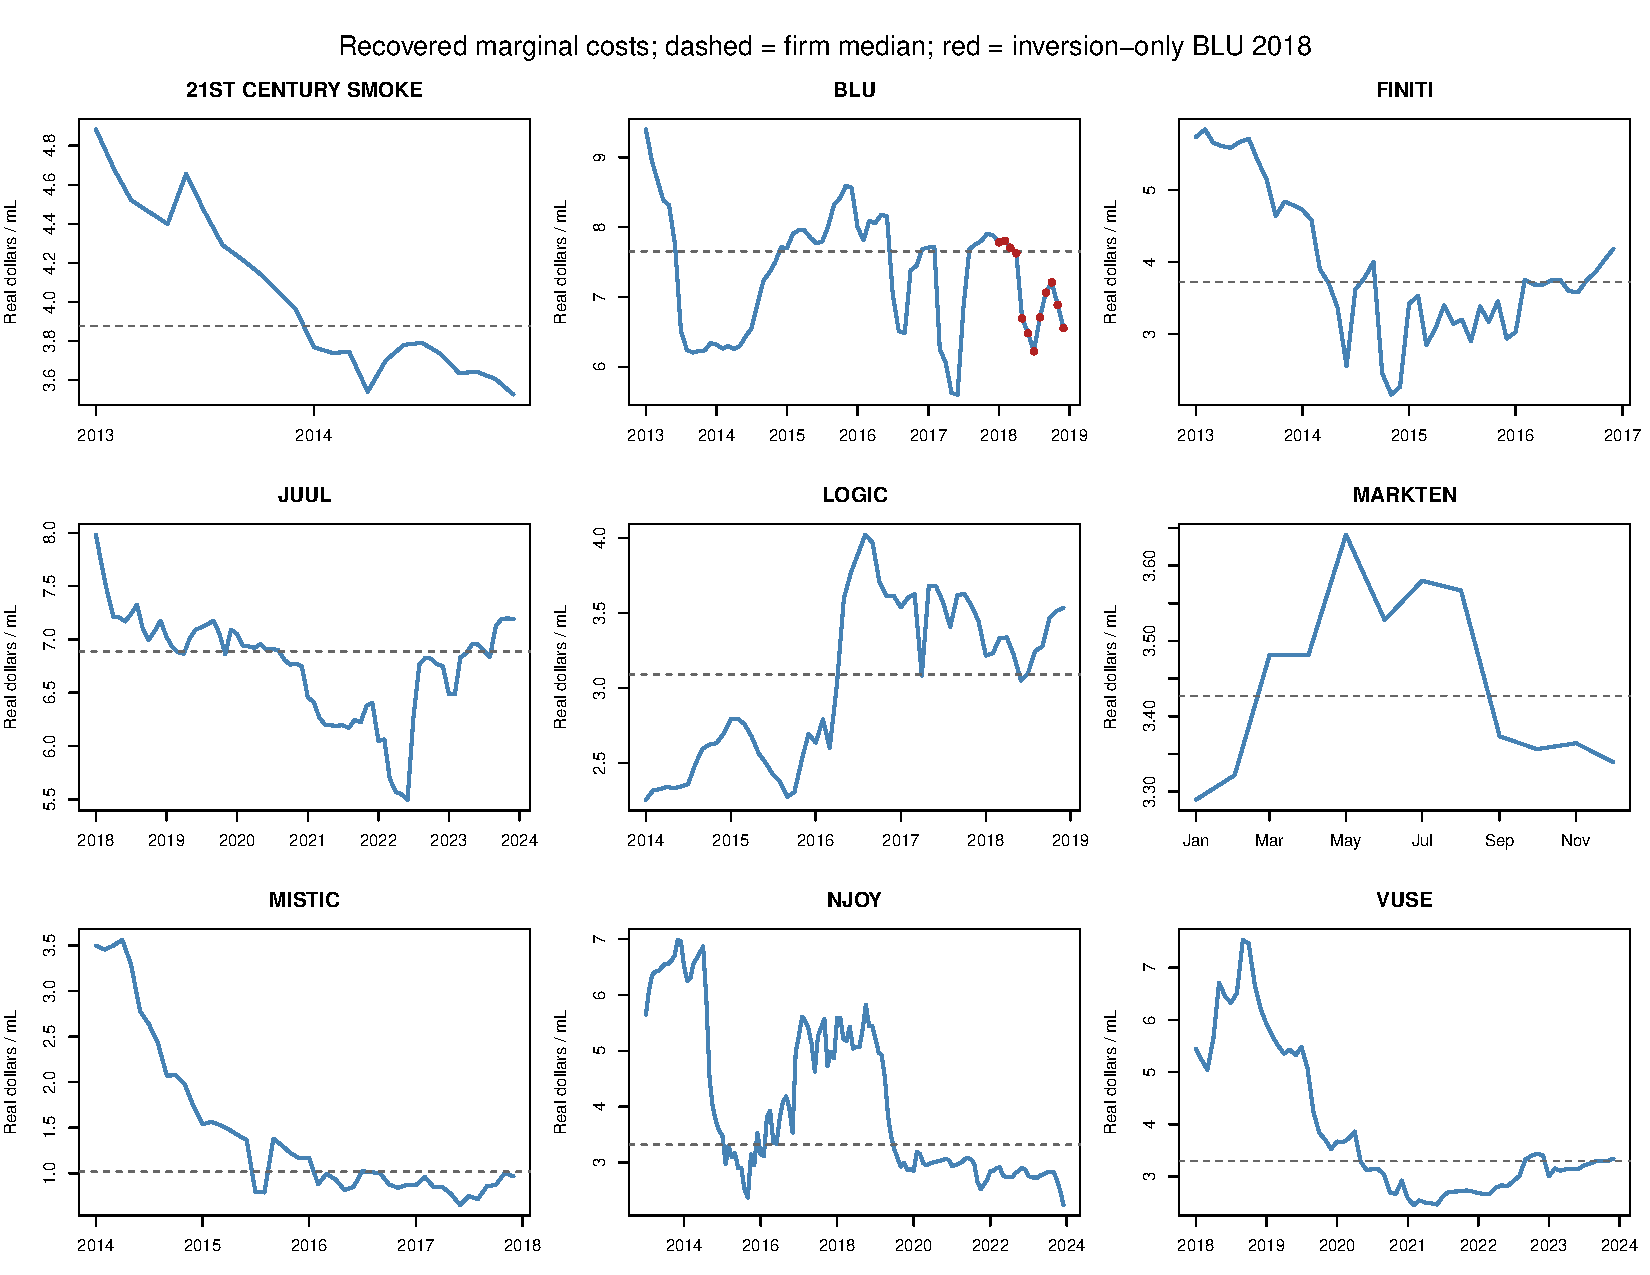
\includepdf[pages=-,landscape=true,fitpaper=true,pagecommand={\thispagestyle{plain}}]{../../output/dynamic_entry_exit/marginal_cost_audit_2026-11-03/recovered_marginal_cost_audit.pdf}

\clearpage

\section{Appendix D. Selected static pricing
audits}\label{appendix-d.-selected-static-pricing-audits}

Next three pages: price/MC/markup time series; convergence from MC +
\$1/mL; unilateral profit curves in a difficult month. These support
pages 3 and 10 without independently validating demand.

\includepdf[pages={3,4,8},landscape=true,fitpaper=true,pagecommand={\thispagestyle{plain}}]{../../output/static_pricing_subgame/manual_fixed_point_2026-10-28/audit/pricing_audit_plots.pdf}

\clearpage

\section{Appendix E. Coordinate-calibration fit
plots}\label{appendix-e.-coordinate-calibration-fit-plots}

Four pages: cumulative entry, survival, active counts, and candidate
losses. Black is observed, blue original trial, red selected calibration
in time-series plots. Search uses 2,000 common-random-number paths; the
separate larger check uses 10,000.

\href{../../output/dynamic_entry_exit/coordinate_search_2026-11-06/candidate_scores.csv}{Candidate
scores}.
\href{../../output/dynamic_entry_exit/coordinate_search_2026-11-06/coordinate_path.csv}{Parameter
path}.
\href{../../output/dynamic_entry_exit/coordinate_search_2026-11-06/independent_simulation_check.csv}{Larger
simulation check}.

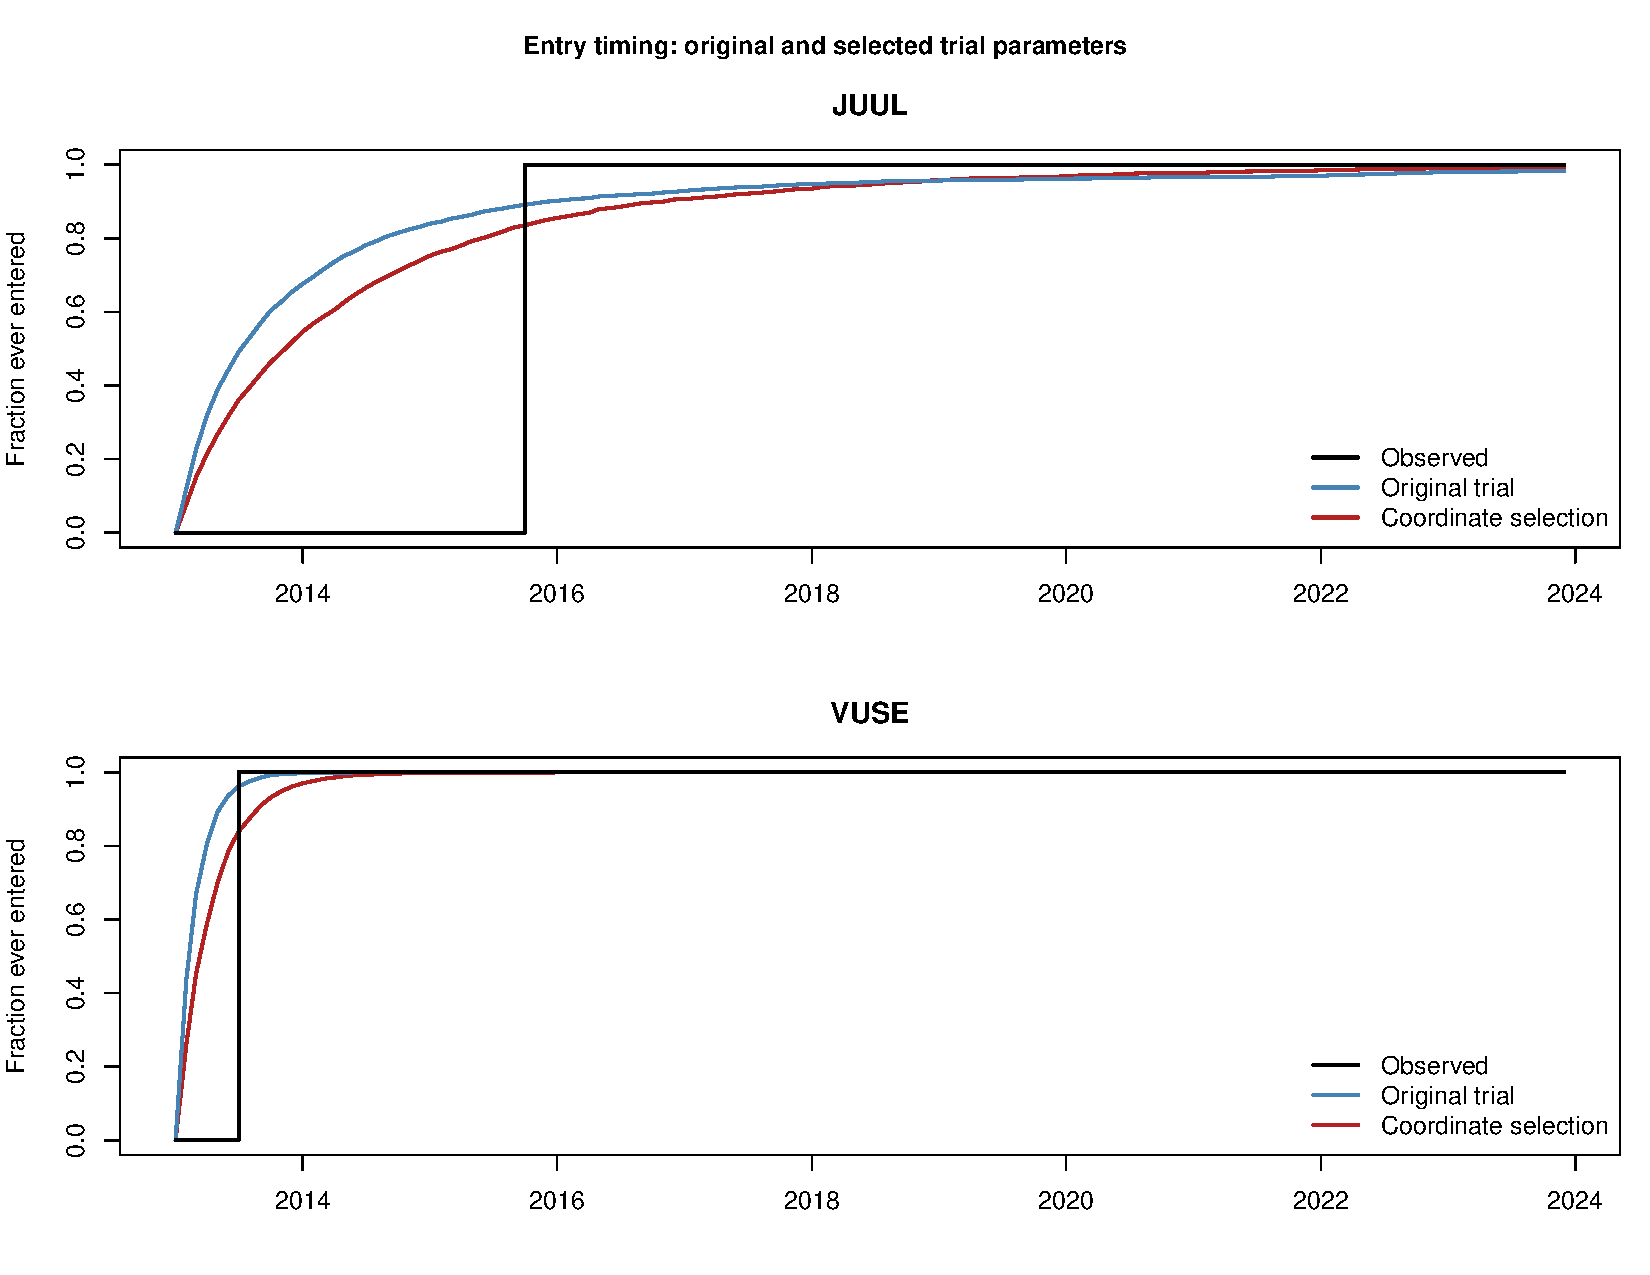
\includepdf[pages=-,landscape=true,fitpaper=true,pagecommand={\thispagestyle{plain}}]{../../output/dynamic_entry_exit/coordinate_search_2026-11-06/coordinate_search_comparison.pdf}

\clearpage

\section{Appendix F. Original dynamic-trial
convergence}\label{appendix-f.-original-dynamic-trial-convergence}

Iteration traces before coordinate calibration. Iterations are
computational updates, not calendar months. Appendix A separately
reports fresh residuals for the selected calibration.

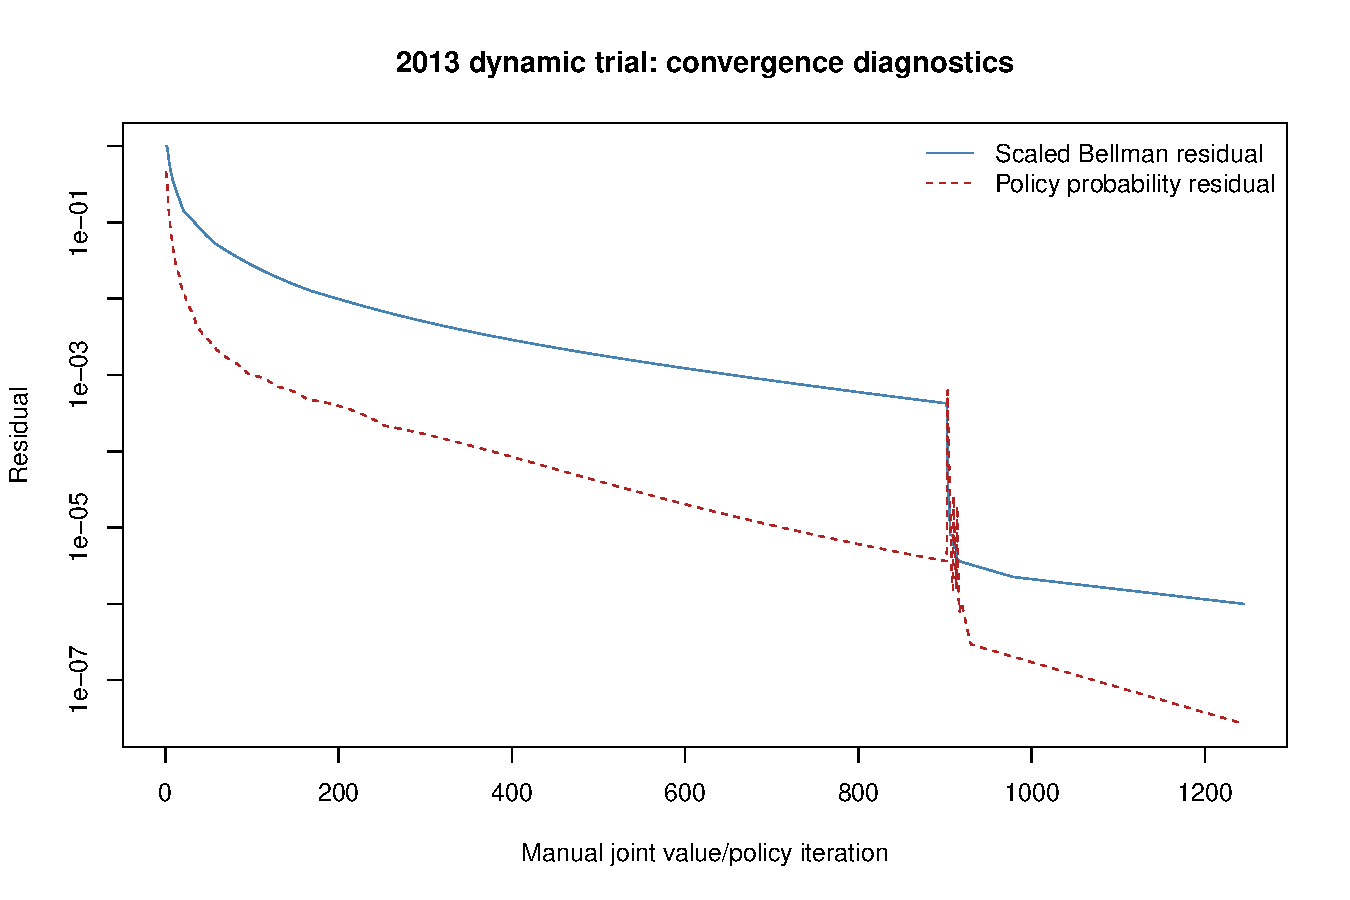
\includepdf[pages=-,landscape=true,fitpaper=true,pagecommand={\thispagestyle{plain}}]{../../output/dynamic_entry_exit/manual_dynamic_trial_2026-11-06/dynamic_convergence.pdf}

\clearpage

\section{Appendix G. From observed shares to simulated
profits}\label{appendix-g.-from-observed-shares-to-simulated-profits}

\textbf{Inverting means solving an equation backward to recover an
unobserved quantity.} Historical recovery and simulated pricing are
separate steps.

\subsection{Step 1: Recover unobserved demand
quality}\label{step-1-recover-unobserved-demand-quality}

Insert observed shares, prices, and nicotine into the estimated demand
equation and solve for its remaining term:

\[
\widehat\xi_{it}=\log(s_{it}/s_{0t})-\widehat c
-\widehat\alpha p_{it}-\widehat\beta_a a_{it}
-\widehat\sigma\log(s_{it}/s_{gt}).
\]

This is the demand residual: the part of mean utility not explained by
the included price and nicotine terms. Using this recovered residual
makes the fitted demand system reproduce observed shares. It does not
independently validate the demand specification.

\subsection{Step 2: Recover historical marginal
cost}\label{step-2-recover-historical-marginal-cost}

Assume the observed price maximizes the specified firm's profit, holding
rivals' prices fixed. Rearrange the pricing FOC:

\[
s_{it}+(p_{it}-mc_{it})\frac{\partial s_{it}}{\partial p_{it}}=0
\quad\Longrightarrow\quad
mc_{it}=p_{it}+\frac{s_{it}}{\partial s_{it}/\partial p_{it}}.
\]

The own-price derivative comes from estimated demand. It is negative, so
implied marginal cost is below price. Historical MC is recovered
separately for each brand-month. The current dynamic baseline then
assigns each brand its historical median cost, held constant across
simulated months and states.

\subsection{Step 3: Calculate profits at a simulated
state}\label{step-3-calculate-profits-at-a-simulated-state}

A simulated state specifies the active roster and each active brand's
nicotine and \(\xi\) bins. With their representative qualities, assigned
costs, and fringe benchmark, solve the pricing game for equilibrium
prices \(p_i^*\) and shares \(s_i^*\).

Quantity is \(q_i^*=Ms_i^*\). Therefore,

\[
\underbrace{(p_i^*-mc_i)Ms_i^*}_{\text{monthly variable profit}}
\; -\; FC
\;=\;\text{monthly operating profit}.
\]

This operating profit enters the continuation/exit problem. Entry costs
and scrap payoffs enter separately at the timing specified on page 7.
Simulated prices are solved using assigned costs; they are not imposed
to equal observed historical prices.

\protect\hyperlink{static-bertrand-pricing-and-recovered-profits}{Return
to static pricing and recovered profits}.

\end{document}
